% Temporarily as a separate document
% Will be placed inside the root latex file

\documentclass[10pt,a4paper]{article}
\usepackage[latin1]{inputenc}
\usepackage{amsmath}
\usepackage{amsthm}
\usepackage{amsfonts}
\usepackage{amssymb}
\usepackage{mathtools}
\usepackage{graphicx}
\usepackage{color}
\usepackage{hyperref}

% theorem environment
\theoremstyle{plain}
\newtheorem{prop}{Proposition}[section]
\newtheorem{theorem}{Theorem}[section]
\newtheorem{cor}{Corollary}[section]
\newtheorem{lem}{Lemma} 
\newtheorem{ex}{Example}
\theoremstyle{definition}
\newtheorem{defn}{Definition}[section]

% For algorithms
\usepackage{algorithm}
\usepackage{algorithmic}

% custom commands
\newcommand{\boldvec}[1]{\boldsymbol{\mathrm{#1}}}
\let\vec\boldvec
\newcommand\at[2]{\left.#1\right|_{#2}} % the at differential sign
\newcommand\scalemath[2]{\scalebox{#1}{\mbox{\ensuremath{\displaystyle #2}}}} % scaling matrices
\DeclareMathOperator{\vect}{vec}

%% custom macros

% % % % Robot control terminology % % % %
\newcommand{\todo}{\textcolor{red}{TODO}} % TODO!
\newcommand{\kin}{\mathcal{T}} % used to denote inverse kinematics
\newcommand{\invKin}{\mathcal{T}^{-1}} % used to denote inverse kinematics

\newcommand{\joint}{\vec{q}} % used to denote robot state in joint space
\newcommand{\state}{\vec{x}} % denotes the generalized coordinates - joint space and velocity coordinates
\newcommand{\error}{\vec{e}} % difference between state and reference
\newcommand{\traj}{\vec{s}} % used to denote the points on the trajectory to be tracked

\newcommand{\dist}{\vec{\epsilon}} % denotes the disturbances acting on the rigid body dynamics
\newcommand{\linDist}{\vec{d}} % denotes the disturbances on the LTV model

\newcommand{\sysInput}{\vec{u}} % used to denote the system inputs
\newcommand{\linInput}{\tilde{\sysInput}} % denotes the LTV inputs
\newcommand{\trjInput}{\vec{\nu}} % denotes the inputs on the trajectory (calculated using IDM)
\newcommand{\ilcInput}{\sysInput_{\mathrm{ILC}}}

% % % % TLS terminology % % % %
\newcommand{\designMat}{\vec{X}} % design matrix
\newcommand{\latentMat}{\vec{Z}} % latent matrix
\newcommand{\observations}{\vec{y}} % observations vector
\newcommand{\fullObs}{\vec{Y}} % observations matrix
\newcommand{\param}{\vec{\beta}} % parameter vector
\newcommand{\fullParam}{\vec{B}} % parameter matrix
\newcommand{\residual}{\vec{r}} % residuals
\newcommand{\weightingMat}{\vec{W}} % weighting the residuals
\newcommand{\errorMat}{\vec{E}} % error matrix
\newcommand{\covarRes}{\vec{\Sigma}_{\residual}} % residual covariance
\newcommand{\leftEigenvector}{\vec{U}} % U of SVD
\newcommand{\rightEigenvector}{\vec{V}} % V of SVD

% % % % ILC terminology % % % %
\newcommand{\qmatrix}{\vec{\Gamma}} % denotes the filtering qmatrix term of Bristow et al.
\newcommand{\lmatrix}{\vec{L}} % denotes the learning matrix of Bristow et al.
\newcommand{\systemMat}{\vec{F}} % system matrix after linearization of f
\newcommand{\dynamics}{\vec{f}}
\newcommand{\dynamicsNominal}{\dynamics_{\mathrm{nom}}}
\newcommand{\policy}{\vec{\pi}}
\newcommand{\ValueFunction}{J}
\newcommand{\episode}{k} % used for episode number
\newcommand{\projOblique}{\vec{P}_{Z,L}^{\perp}} % used for oblique projection
\newcommand{\projOrth}{\vec{P}_{Z}^{\perp}} % used for orthogonal projection perp. to ran(Z)
\newcommand{\proj}{\vec{P}_{Z}} % used for orthogonal projection to ran(Z)

\newcommand{\totalTime}{T} % total time duration 
\newcommand{\numSteps}{N} % total number of time steps
\newcommand{\numepisode}{K} % total number of episodes

\newcommand{\threshold}{\epsilon}
\newcommand{\alg}{\emph{tILC}}
\newcommand{\dataset}{E}

\newcommand\red[1]{{\color{red}#1}}
\newcommand\blue[1]{{\color{blue}#1}}
\newcommand\bluebold[1]{\textbf{{\color{blue}#1}}}
\newcommand\gray[1]{{\color{gray}#1}}

% Set the paths where all figures are taken from:
\graphicspath{{Pictures/}}
\mathtoolsset{showonlyrefs} 
\newcommand{\includesvg}[1]{%
% \executeiffilenewer{#1.svg}{#1.pdf}%
% {inkscape -z -D --file=#1.svg %
% --export-pdf=#1.pdf --export-latex}%
 \input{#1.pdf_tex}%
}

\author{Okan Ko\c c, Guilherme Maeda and Jan Peters}
\title{Cautious Learning Control with Total Least Squares}
\begin{document}

\maketitle
\thispagestyle{empty}
\pagestyle{empty}

%%%%%%%%%%%%%%%%%%%%%%%%%%%%%%%%%%%%%%%%%%%%%%%%%%%%%%%%%%%%%%%%%%%%%%%%%%%
\begin{abstract}

Iterative Learning Control is a control theoretic learning paradigm that aims to iteratively improve the tracking performance of a repetitive system. Optimization based approaches to ILC assume that a detailed knowledge of the plant to be controlled is available. However, such approaches can diverge terribly due to overconfidence. 

In this paper, we propose a more cautious ILC algorithm using Total Least Squares (TLS), that is robust with respect to modeling uncertainties. We prove that our algorithm is monotonically convergent for a wider range of nominal models, compared to existing model-based approaches. Moreover we give a Bayesian interpretation of TLS and build an adaptive routine that can adaptively identify the underlying linearized model. Simulation and real robot results confirm the practical significance of our contributions. %incrementally or iteratively identify?
\end{abstract}

%%%%%%%%%%%%%%%%%%%%%%%%%%%%%%%%%%%%%%%%%%%%%%%%%%%%%%%%%%%%%%%%%%%%%%%%%%%


\section{Introduction}

% RC reference needed
Learning Control paradigms, and in particular Iterative Learning Control (ILC) \cite{Arimoto84}, \cite{Bristow06} and Repetitive Control (RC) \cite{Wang09}, \cite{Longman2000}, aim to iteratively improve the tracking performance of a control system subject to repetitive tasks. In ILC, these tasks are episodic in nature: follow a desired trajectory for a fixed time duration and repeat after resetting to a certain initial state. The feedforward control inputs are adjusted based on the resulting deviations from the reference. In RC, on the other hand, the reference trajectory is periodic and tracked continuously, and unlike ILC, no resetting occurs.
%In ILC, usually the feedforward control inputs are adjusted after each trial based on the resulting deviations from the reference trajectory. The goal is to drive such deviations to zero. 

Methods that learn to track (periodic or episodic) trajectories need to compensate for modeling uncertainties and other repetitive disturbances acting on the system to be controlled. However, stable methods that can efficiently and safely learn the dynamics are model-based (e.g. most of optimization-based ILC \cite{Amann95},\cite{Bristow06}) and at least require a global understanding of the dynamics of the system \cite{Kolter09}, \cite{NguyenTuong11}.
% some more references here, on model based policy search for example?

% refs needed
When executing model-based learning algorithms on dynamic systems, it is essential for stability and safety to incorporate a notion of model uncertainty. Otherwise the learning algorithms can be overconfident and quickly go unstable~\cite{Longman2000}. One way to achieve a more stable performance is to use regularization. For example, in ILC, the inputs or the change in inputs applied to a system can be penalized. These robust methods in ILC are mostly known as Q-filtering~\cite{Bristow06} and typically incur a trade-off between stability and performance: system will often converge to a nonzero steady-state error. % if the learning algorithm is agnostic to the true dynamics of the system, it will fail to converge to zero steady-state error.

% is it the stability margin? or simply monotonic convergence?
In this paper, we introduce another way to increase the stability margins of model-based ILC that does not incur such a trade-off. We treat the modelling uncertainty issue in an errors-in-variables regression context and use in particular Total Least Squares (TLS) \cite{Golub80} to perform the ILC updates. By adjusting the feedforward control inputs with the TLS regressor, we exercise caution and ensure robustness with respect to model uncertainty. % while at the same time improving the steady-state performance. 

Our contributions to Learning Control can be summarized as follows:

\begin{itemize}
\item We form a link between model-based Learning Control methods and errors-in-variables regression models, and analyze in particular Total Least Squares (TLS).
\item We prove that we increase the stability margins (in the iteration domain) of ILC by incorporating a truncated TLS update rule, and ensure monotonic convergence without sacrificing minimal steady-state error. 
\item We exploit the structure of the block lower triangular matrix estimation problem within TLS and increase its applicability for control problems. Simulation and real robot experimental results are presented.
\item We show as an extension of our ideas, one way to incorporate a Bayesian update rule within TLS and achieve self-tuning property. 
% relation to Kalman filter and other methods? Higher order ILC?
\end{itemize}

The outline of the paper is as follows: in the next subsection \ref{relatedWork} we give a brief literature review related to our work. In section \ref{methodology} we start by analyzing Total Least Squares. We present truncated structured TLS, along with pseudocode, and show its applicability in Iterative Learning Control. The resulting algorithm $\alg$ with minor modifications can be applied to Repetitive Control (RC) as well. In subsection \ref{ilcTLS} we prove the monotonic convergence and minimal steady state error of $\alg$. An adaptive version of $\alg$ is presented in \ref{adaptiveILC}, simulation results and real robot experiments are given in \ref{results}. Finally, conclusions and brief mention of possible future directions to explore are given in \ref{conclusions}.

% references required as always.  
\subsection{Related Work}\label{relatedWork}

A thorough investigation of the statistical properties of Total Least Squares (TLS) as well as its extensions such as structured TLS are presented in \cite{VanHuffel91}. For a short overview see \cite{Golub80} or the Appendix in \cite{Golub96}. Literature on TLS is huge and the application areas are growing rapidly. For some of the applications of TLS and errors-in-variables modelling, see the recent book \cite{VanHuffel13}. Truncated total least squares as a regularization method~\cite{Fierro97} is widely used in practice. % ref?
% relation to PCA? refs?

One of the first papers that introduced Iterative Learning Control (ILC) is \cite{Arimoto84}. For a good survey, see \cite{Bristow06} or \cite{Moore07}. Desirable properties of ILC algorithms include stability and monotonicity, and are discussed, for example, in \cite{Norrloef02} and \cite{Bristow06}. Optimization based ILC is described, for example, in \cite{Amann95}, \cite{Bristow06}, \cite{Moore07}. It seems we are not the first to notice the connection between ILC and TLS: another application of TLS in ILC using Tikhonov regularization~\cite{Golub99} is given in \cite{ZhangBo14}. In this work we use instead truncated total least squares (TTLS).

% % 2D systems analysis reference?
% % More applications of TLS? Especially in system identification, modelling, signal processing, etc.
% % Repetitive Control??
% % Shall we mention the ILC in nonlinear control systems review?

\section{Methodology}\label{methodology}

In this section we start by fixing the notation that we use for regression. We introduce more control-theoretic notation as we go along.
%
\subsection{Linear Least Squares}
Let $\designMat \in \mathbb{R}^{m \times n}$ be the design matrix, $\observations \in \mathbb{R}^{m}$ the vector of observations and  $\param \in \mathbb{R}^{n}$ the parameter vector to be estimated: $\designMat\param \approx \observations$. In this linear regression model $\residual = \observations - \designMat\param$ are the residuals that are to be minimized with respect to 2-norm~\cite{Golub80}
%
\begin{equation}
\begin{aligned}
\text{minimize} &\ \residual^{\mathrm{T}}\weightingMat\residual, \\
\text{subject to} &\ \observations + \residual \in \text{Range}(\designMat).
\end{aligned}
\label{lls}
\end{equation}
%
\noindent The weight matrix $\weightingMat$ is chosen to be positive definite and ideally should be the inverse of the covariance matrix $\covarRes$ of the residuals. The well-known \emph{normal equations} $\designMat^{\mathrm{T}}\weightingMat\designMat \param = \designMat^{\mathrm{T}} \weightingMat\observations$ provide the unique closed-form solution to this problem in case $\designMat$ is of full rank, $\text{rank}(\designMat) = n$. Solution to the normal equations can then be computed in a numerically stable way~\cite{Golub96} using e.g. QR decomposition methods. If the design matrix $\designMat$ is of low rank, pseudoinverse $\designMat^{\dagger}$ finds out of infinitely many solutions the minimum 2-norm solution $\hat{\param} = \designMat^{\dagger}\observations$ and can be computed using SVD. % this should be verified. [see Golub'96]

In case the design matrix $\designMat$ is numerically rank-deficient (i.e. its condition number is large), ridge regression (i.e. Tikhonov regularization) or truncation methods can be used to regularize (and hence to come up with a numerically stable estimate of) the parameter $\param$ in \eqref{lls}. Truncation can be applied conveniently with the pseudoinverse: invert the large singular values of $\designMat$ above a certain user-specified threshold $\threshold$ and truncate the rest to zero.

\subsection{Total Least Squares: an errors-in-variables model}
% shall we use multiple right hand sides?
% include weighting in the derivation?

Total Least Squares (TLS) is an errors-in-variables model that is applicable when the design matrix $\designMat$ is also not precisely known,
i.e. $(\designMat + \errorMat)\param = \observations + \residual$ for an unknown $\errorMat$ hopefully with small norm. A Frobenius-norm optimization procedure with diagonal weighting matrices $\weightingMat_{L} \in \mathbb{R}^{m \times m}$ and $\weightingMat_{R} \in \mathbb{R}^{n+1 \times n+1}$ is a natural extension of \ref{lls} under this model
%
\begin{equation}
\begin{aligned}
\text{minimize} &\ \| \weightingMat_{L} \begin{bmatrix} \errorMat & \residual \end{bmatrix} \weightingMat_{R} \|_{F}, \\
\text{subject to} &\ \observations + \residual \in \text{Range}(\designMat + \errorMat).
\end{aligned}
\label{tls}
\end{equation}
%
\noindent The singular-value decomposition (SVD) based solution to \eqref{tls} is described in \cite{Golub80} \footnote{However in general \ref{tls} fails to have a solution. An example with low-rank design matrix can be found in \cite{Golub80}} and relies on the Eckart-Young theorem. We show here for convenience the case where the weighting matrices $\weightingMat_{L}$ and $\weightingMat_{R}$ are identity. Rewriting $(\designMat + \errorMat)\param = \observations + \residual$ as  
%
\begin{equation}
\begin{aligned}
\begin{bmatrix} \designMat + \errorMat & \observations + \residual \end{bmatrix} \begin{bmatrix} \param \\ -1 \end{bmatrix} = 0, \\
\end{aligned}
\end{equation}
%
\noindent and using the Eckart-Young decomposition for a minimum Frobenius norm matrix $\begin{bmatrix} \hat{\errorMat} & \hat{\residual} \end{bmatrix}$% reference needed 
%

\begin{align}
\begin{bmatrix} \designMat & \observations \end{bmatrix} = \begin{bmatrix} \leftEigenvector_{X} & \vec{u}_{y} \end{bmatrix} \begin{bmatrix} \vec{\Sigma}_{X} & 0 \\ 0 & \sigma_{y} \end{bmatrix} \begin{bmatrix} \rightEigenvector_{XX} & \vec{v}_{Xy} \\ \vec{v}_{yX} & v_{yy} \end{bmatrix}^{\mathrm{T}}, \label{eckart1} \\
\begin{bmatrix} \designMat + \hat{\errorMat} & \observations + \hat{\residual} \end{bmatrix} = \begin{bmatrix} \leftEigenvector_{X} & \vec{u}_{y} \end{bmatrix} \begin{bmatrix} \vec{\Sigma}_{X} & 0 \\ 0 & 0 \end{bmatrix} \begin{bmatrix} \rightEigenvector_{XX} & \vec{v}_{Xy} \\ \vec{v}_{yX} & v_{yy} \end{bmatrix}^{\mathrm{T}} \label{eckart2}.
\end{align}
% 
\noindent After subtracting \eqref{eckart2} from \eqref{eckart1} and manipulating we get
%
\begin{align}
\hat{\param}_{tls} &= -\frac{\vec{v}_{Xy}}{v_{yy}}, \label{tls1} \\
\hat{\errorMat} &= \leftEigenvector_{X} \vec{\Sigma}_{X} \rightEigenvector_{XX}^{\mathrm{T}} - \designMat. \label{tls2}
\end{align}

\noindent The SVD solution nicely separates the parameter estimate $\hat{\param}$ from the \emph{latent matrix} estimate $\hat{\latentMat} = \designMat + \hat{\errorMat} = \leftEigenvector_{X} \vec{\Sigma}_{X} \rightEigenvector_{XX}^{\mathrm{T}}$. See Figure~\ref{Figure1} for an illustration in one-dimensional regression. The case for multiple right-hand sides (i.e. $\observations \in \mathbb{R}^{n \times k}, k > 1$) and diagonal weighting matrices is given in \cite{Golub96}. Further extensions including partial, global, structured, and truncated TLS can be found in \cite{VanHuffel91}. 
% more citations are necessary!
% mention that we are extracting a latent dynamics matrix F_est = F + E!
Pseudocode for a general structured and truncated total least squares algorithm implementing an SVD solution is given in Algorithm~\ref{alg1}. Notation is adapted slightly for the general case. The latent matrix estimation step is made explicit. % refer to latent matrix estimation (PCA?) literature.

\begin{figure}
\centering
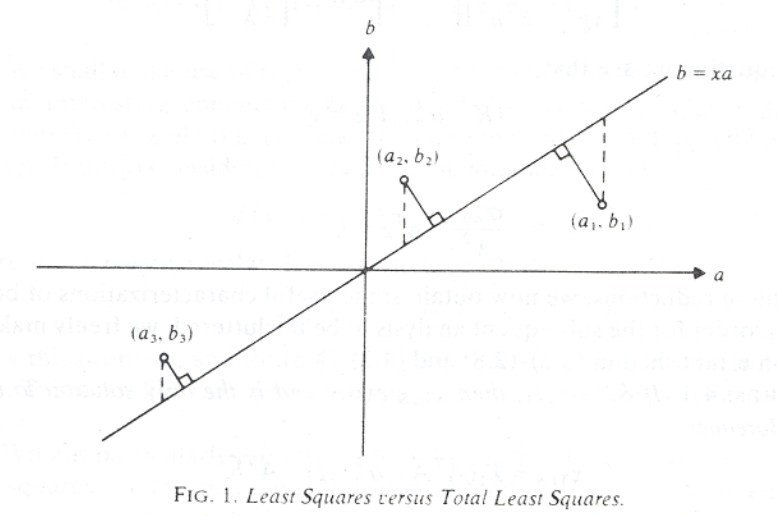
\includegraphics[width=0.4\textwidth]{LSvsTLS.jpg}%
\caption{Comparison between least squares and total least squares in the one dimensional estimation setting, taken from \cite{Golub80}. Least Squares minimizes the sum of the squared vertical distances from observations to the regression line. Total Least Squares is also known as orthogonal regression in 1D and minimizes instead the sum of the squared perpendicular distances.}
\label{Figure1}
\end{figure}
%

\begin{algorithm}[tb]
   \caption{Structured Truncated Total Least Squares}
   \label{alg1}
\begin{algorithmic}
   \STATE {\bfseries Input:} $\threshold > 0$, $\designMat$, $\fullObs = \begin{bmatrix} \observations_1 & \observations_2 & \ldots & \observations_k \end{bmatrix}$, $\weightingMat_{L}$, $\weightingMat_{R} = \begin{bmatrix} \weightingMat_{R1} & \weightingMat_{R2}\end{bmatrix}$.
   \STATE Compute SVD solution $\leftEigenvector \vec{\Sigma} \rightEigenvector^{\mathrm{T}} = \weightingMat_{L}\begin{bmatrix} \designMat & \fullObs \end{bmatrix}\weightingMat_{R}$.
   \STATE Estimate parameter $\hat{\fullParam} = -\weightingMat_{R1}\vec{V}_{XY}\vec{V}_{YY}^{-1}\weightingMat_{R2}^{-1}$.
   \STATE Estimate latent matrix $\hat{\latentMat} = \leftEigenvector_{X} \vec{\Sigma}_{X} \rightEigenvector_{XX}^{\mathrm{T}}$.
\end{algorithmic}
\end{algorithm}

%
\subsection{Iterative Learning Control with Total Least Squares}\label{ilcTLS}
%
In Iterative Learning Control (ILC) the goal is to drive deviations from a fixed reference trajectory $\traj(t), \ 0 \leq t \leq T \ $ in state space $\state \in S \subset \mathbb{R}^{p}$ to zero when the system to be controlled is subject to unknown repeating disturbances and model mismatch \cite{Bristow06}. As opposed to other adaptive (learning) control approaches, in ILC usually the feedforward control inputs to the system $\sysInput(t)$ are adjusted after each iteration $k$, or episode, is completed and the resulting deviations $\error(t) = \state(t) - \traj(t)$ from the desired trajectory are observed. % references to adaptive control literature?

Consider a general nonlinear dynamical system governed by the differential equation
%
\begin{align}
\dot{\state} &= \dynamics(\state,\sysInput), \label{dynamics} \\
\dot{\state} &= \dynamicsNominal(\state,\sysInput) + \dist(\state,\sysInput). \label{dynamicsNom}
\end{align}
%
% reference to other nonlinear approaches to ILC?
\noindent Assume that the nominal model $\dynamicsNominal$ is all we know about the system in \eqref{dynamics}. Nonlinear approaches to ILC mostly consider linearizations of \eqref{dynamicsNom} around the trajectory $\traj(t)$ and nominal inputs $\trjInput(t)$. Discretizing and stacking the linear time varying matrices obtained, we get the following \emph{lifted-form} approximation of the underlying dynamics
%
\begin{equation}
\begin{aligned}
\error \approx \systemMat \sysInput - \linDist,
\end{aligned}
\label{approxModel}
\end{equation}
%
\noindent where the model matrix $\systemMat$ has a block lower-diagonal structure, and is composed of the submatrices
%
\begin{equation}
\begin{aligned}
\vec{F}_{(i,j)} &= \left \{
\begin{array}{cc}
\vec{A}_{i-1}\ldots \vec{A}_j \vec{B}_{j-1}, & j < i, \\ 
\vec{B}_{j-1}, & j = i, \\
\vec{0}, & j > i. 
\end{array} \right.
\end{aligned}
\label{Fmatrix}
\end{equation}

\noindent Matrices $\vec{A}_j$ and $\vec{B}_j$ are linearizations of the nominal model $\dynamicsNominal$ around the discrete trajectory points $\traj_j$ and nominal inputs $\vec{\nu}_j$ respectively. Conventional ILC algorithms using such a linearized model compute at each iteration the feedforward compensation signals $\sysInput = (\sysInput_1^{\mathrm{T}}, \ldots, \sysInput_N^{\mathrm{T}})^{\mathrm{T}}$ and add to nominal input $\trjInput = (\trjInput_1^{\mathrm{T}}, \ldots, \trjInput_N^{\mathrm{T}})^{\mathrm{T}}$ to drive error $\error = (\error_1^{\mathrm{T}}, \ldots, \error_N^{\mathrm{T}})^{\mathrm{T}}$ to minimum achievable error (ideally zero). For example, the ILC algorithm utilizing plant inversion with pseudoinverse computes the updates using % ref needed
% 
%
\begin{equation}
\begin{aligned}
\sysInput_{k} = \systemMat^{\dagger}\linDist_{k},
\end{aligned}
\label{pseudoinverseILC1}
\end{equation}
%
\noindent where $\linDist_{k}$ is estimated using the last iteration $k-1$, i.e. $\linDist_{k} \approx \systemMat \sysInput_{k-1} - \error_{k-1}$. Putting it all together, when the system matrix $\systemMat$ is of full rank, we get the following model-based ILC update law 
%
\begin{equation}
\begin{aligned}
\sysInput_{k+1} = \sysInput_{k} - \systemMat^{\dagger}\error_{k}.
\end{aligned}
\label{pseudoinverseILC2}
\end{equation}
%
\noindent In MATLAB the command for computing \eqref{pseudoinverseILC2} with truncation parameter $\epsilon$ is \emph{pinv}$(\designMat,\epsilon)$ where the singular values of $\designMat$ less than $\epsilon$ are treated as zero. 

The compensations in \eqref{pseudoinverseILC2} are computed using the approximate model in \eqref{approxModel} and should be instead computed more cautiously. In particular, it is not enough to state that the control inputs will eventually converge to a steady-state value, as is often done when proving the \emph{stability} of ILC algorithms. For practical and for safety purposes one needs to also ensure that the errors incurred along the trajectory at each iteration are decreasing, under a particular vector norm. This is studied in the ILC literature as the \emph{monotonic convergence} criterion~\cite{Bristow06}. 

We take the monotonic convergence criterion into account by using Total Least Squares to come up with a more cautious ILC update. Combining \eqref{pseudoinverseILC2} and \eqref{tls} we get $\alg$
%
\begin{align}
\sysInput_{k+1} &= \sysInput_{k} - \delta \sysInput_{k}, \label{tlsilc1} \\ 
\delta \sysInput_{k}, \ \hat{\errorMat}_k &= \arg\min \|\begin{bmatrix}\errorMat_k & \residual_k \end{bmatrix} \|_{F}, \label{tlsilc2} \\
\text{subject to} &\ (\systemMat + \errorMat_k)\delta \sysInput_k = \error_k + \residual_k \label{tlsilc3}.
\end{align}
%

\subsection{Monotonic Convergence}\label{monotonic}

In this section we analyze and prove the monotonic convergence of the pseudoinverse-based ILC in \eqref{pseudoinverseILC2} and TLS-based ILC in \eqref{tlsilc2} under certain conditions. These conditions will be seen to be more restrictive for pseudoinverse-based ILC. Furthermore, we indicate the effects of truncated and structured TLS solutions to convergence and stability. For the readers convenience, we will be as self-contained as possible. We consider the usual Euclidian norm, i.e the 2-norm, as our vector norm $\|\cdot\|$. We start by analyzing the conditions for stability in the iteration domain. 

% first order vs. higher order?
% Q matrix?
\begin{defn} An ILC update law of the form $\sysInput_{k+1} = \sysInput_{k} - \lmatrix \error_{k}$ with $\lmatrix \in \mathbb{R}^{n \times m}$ operating on the unknown system with response $\error = \latentMat \sysInput + \linDist$ is said to be \emph{asymptotically stable} in the iteration-domain if the control inputs are bounded: $\exists M \in \mathbb{R} \ $ s.t. $\ \|\sysInput_k\| < M, \ \forall k \in \mathbb{Z}^{+}$ and the limit exists: $\lim\limits_{k \to \infty}\sysInput_k = \sysInput_{\infty} \in \mathbb{R}^{n}$. \end{defn}
%
We refer to the input-output matrix $\latentMat$ of the unknown system as the \emph{latent matrix} and $\lmatrix$ as the \emph{learning matrix}. Conditions for ensuring asymptotic stability are given below.
%
\begin{lem}[AS] \label{AS} A system operating under an ILC update law is asymptotically stable (AS) if the spectral radius $\rho = |\lambda_{\mathrm{max}}(\vec{I} - \lmatrix\latentMat)| < 1$. \end{lem}
%
\begin{proof}
Taking the dynamics $\error = \latentMat \sysInput + \linDist$ for an arbitrary initial guess $\sysInput_0 \in \mathbb{R}^{n}$
\begin{align}
\sysInput_1 &= \sysInput_0 - \lmatrix\error_0 = (\vec{I} - \lmatrix\latentMat)\sysInput_0 - \lmatrix\linDist, \\
\sysInput_2 &= \sysInput_1 - \lmatrix(\latentMat\sysInput_1 + \linDist) = (\vec{I} - \lmatrix\latentMat)^{2}\sysInput_0 - (\vec{I} - \lmatrix\latentMat)\lmatrix\linDist - \lmatrix\linDist.
\end{align}
%
\noindent Hence for an arbitrary $k \in \mathbb{Z}^{+}$
%
\begin{align}
\sysInput_{k+1} &= (\vec{I} - \lmatrix\latentMat)\sysInput_{k} - \lmatrix\linDist, \\
\sysInput_k &= (\vec{I} - \lmatrix\latentMat)^{k}\sysInput_0 - \Big(\sum_{l=0}^{k-1}(\vec{I} - \lmatrix\latentMat)^{l}\Big)\lmatrix\linDist.
\end{align}
%
\noindent The series $\{\sysInput_{k}\}_{k=1}^{\infty}$ is bounded and convergent if and only if the spectral radius $\rho < 1$. Moreover the matrix $\lmatrix\latentMat$ is invertible since we can find a matrix norm $\|\cdot\|$ with $\rho \leq \|\vec{I} - \lmatrix\latentMat\| \leq \rho + \delta$ for some $\delta < 1 - \rho$ which implies $(\lmatrix\latentMat)^{-1} = \sum_{l=0}^{\infty}(\vec{I} - \lmatrix\latentMat)^{l}$. The limit is the fixed point of the series
% put reference for invertibility
%
\begin{align}
\sysInput_{\infty} &= (\vec{I} - \lmatrix\latentMat)\sysInput_{\infty} - \lmatrix\linDist, \\
\sysInput_{\infty} &= -(\lmatrix\latentMat)^{-1}\lmatrix\linDist.
\end{align}
%
\end{proof}
%
We can now easily show the steady-state error of the ILC law.
%
\begin{cor}
For a system that is asymptotically stable in the iteration-domain, the steady-state error is finite: $\error_{\infty} = (\vec{I} - \latentMat(\lmatrix\latentMat)^{-1}\lmatrix)\linDist$. In particular, $\projOblique = (\vec{I} - \latentMat(\lmatrix\latentMat)^{-1}\lmatrix)$ is an oblique projection matrix onto $\mathrm{null}(\latentMat^{\mathrm{T}})$ and is orthogonal if $\lmatrix = \latentMat^{\dagger}$.
\end{cor}
%
\begin{proof}
%
\begin{align}
\error_{\infty} &= \latentMat\sysInput_{\infty} + \linDist, \\
\error_{\infty} &= -\latentMat(\lmatrix\latentMat)^{-1}\lmatrix\linDist + \linDist = (\vec{I} - \latentMat(\lmatrix\latentMat)^{-1}\lmatrix)\linDist.
\end{align}
%
Conditions for the projection matrix can be easily checked.
\end{proof}
%
The corollary states that to get a steady-state error of smallest norm, we would need to know the exact dynamics of the system. However, even without knowing the exact dynamics, conditions for asymptotic stability are easy to satisfy. %
With Lemma~\ref{AS} it is difficult to come up with a constructive criterion for AS however. Especially we would like to obtain a more easily checked AS criterion for the pseudoinverse of $\systemMat$ when the underlying system $\latentMat$ is close to $\systemMat$, e.g. $\latentMat = \systemMat + \errorMat$ for some error $\errorMat$ with bounded spectral norm, $\|\errorMat\|_2 < M$, with $M \in \mathbb{R}$ small. We now give such a (sufficient) criterion for AS.
%
\begin{lem}
A system operating under the pseudoinverse update law \eqref{pseudoinverseILC2} is asymptotically stable (AS) if the matrices $\systemMat$, $\latentMat$ are full rank, i.e. $\mathrm{rank}(\systemMat) = \mathrm{rank}(\latentMat) = n$ and $\|\errorMat\|_2 = \sigma_{max}(\errorMat) < \sigma_{min}(\systemMat) = 1/\|\systemMat^{\dagger}\|_2$.
\end{lem}
%
\begin{proof}
It is sufficient to bound the spectral radius with the spectral norm and show that it is less than one. The fact that $\systemMat$ is of full column rank simplifies things quite significantly. Using $\systemMat^{\dagger}\systemMat = \vec{I}$
%
\begin{align}
\rho(\vec{I} - \lmatrix\latentMat) \leq \|\vec{I} - \lmatrix\latentMat\|_2 = \|\vec{I} - \systemMat^{\dagger}(\systemMat + \errorMat)\|_2 =  \|\systemMat^{\dagger}\errorMat\|_2 \leq \|\systemMat^{\dagger}\|_2\|\errorMat\|_2,
\end{align}
%
which is less than one if $\|\errorMat\|_2 < 1/\|\systemMat^{\dagger}\|_2$.
\end{proof}
%
Generally an asymptotically stable ILC algorithm may not be \emph{monotonic}.
%
\begin{defn}
An AS system operating under an ILC update law is monotonically convergent (MC) with rate $1/\gamma$, $0 < \gamma < 1$, if $\|\error_{k+1} - \error_{\infty}\| < \gamma \|\error_{k} - \error_{\infty}\|$ for all $k \in \mathbb{Z}^{+}$.
\end{defn}
%
The bounds on the error matrix $\errorMat$ guaranteeing MC are much tighter than bounds for AS.
%
\begin{lem} The ILC update law of the form $\sysInput_{k+1} = \sysInput_{k} - \lmatrix \error_{k}$ with $\lmatrix = \systemMat^{\dagger}$ operating on the unknown system with response $\error = \latentMat \sysInput + \linDist$ is monotonically convergent under the spectral norm with rate $1/\gamma$, $\gamma < 1$ if the matrices $\systemMat$, $\latentMat = \systemMat + \errorMat$ are full rank and $\|\errorMat\|_2 = \sigma_{max}(\errorMat) < \frac{\gamma\sigma_{min}^{2}(\systemMat)}{\mu\sigma_{max}(\systemMat) + \mu\sigma_{min}(\systemMat) + \gamma\sigma_{min}(\systemMat)}$, $\mu = \frac{1 + \sqrt{5}}{2}$.  \end{lem}
%
\begin{proof}
Writing again the dynamics equation and iterating with the ILC law we get
%
\begin{align}
&\error_{k+1} = \latentMat(\sysInput_k - \lmatrix\error_k) + \linDist, \\
&\error_{k+1} = \error_{k} - \latentMat\lmatrix\error_k = (\vec{I} - \latentMat\lmatrix)\error_k, \\
&\error_{k+1} - \error_{\infty} = (\vec{I} - \latentMat\lmatrix)\error_k - (\vec{I} - \latentMat(\lmatrix\latentMat)^{-1}\lmatrix)\error_k, \\
&\error_{k+1} - \error_{\infty} = (\latentMat\lmatrix - \latentMat(\lmatrix\latentMat)^{-1}\lmatrix)\error_k, \\
&\error_{k} - \error_{\infty} = \latentMat(\lmatrix\latentMat)^{-1}\lmatrix\error_k,
\end{align}
%
Since the system is AS according to Lemma~\ref{AS} and the inverse of $\lmatrix\latentMat$ exists, $\vec{I} = \lmatrix\latentMat(\lmatrix\latentMat)^{-1}$ and
%
\begin{align}
\|\error_{k+1} - \error_{\infty}\|_2 &= (\latentMat\lmatrix\latentMat(\lmatrix\latentMat)^{-1}\lmatrix - \latentMat(\lmatrix\latentMat)^{-1}\lmatrix)\error_k, \\
\|\error_{k+1} - \error_{\infty}\|_2 &= \|(\vec{I} - \latentMat\lmatrix)\latentMat(\lmatrix\latentMat)^{-1}\lmatrix\error_k\|_2, \\
\|\error_{k+1} - \error_{\infty}\|_2 &= \|(\vec{I} - \latentMat\latentMat^{\dagger})\latentMat(\lmatrix\latentMat)^{-1}\lmatrix\error_k - \latentMat(\lmatrix - \latentMat^{\dagger})\latentMat(\lmatrix\latentMat)^{-1}\lmatrix\error_k\|_2, \\
\|\error_{k+1} - \error_{\infty}\|_2 &= \|\latentMat(\systemMat^{\dagger} - \latentMat^{\dagger})\latentMat(\lmatrix\latentMat)^{-1}\lmatrix\error_k\|_2,
\end{align}
%
since $\latentMat\latentMat^{\dagger}\latentMat = \latentMat$. The matrix 2-norm is an induced norm and compatible by definition
%
\begin{align}
\|\error_{k+1} - \error_{\infty}\|_2 &\leq \|\latentMat\|_2\|\systemMat^{\dagger} - \latentMat^{\dagger}\|_2\|\error_{k} - \error_{\infty}\|_2,\\
%\|\error_{k+1} - \error_{\infty}\|_2 &< \gamma\|\error_{k} - \error_{\infty}\|_2,
\end{align}
%
We can use e.g. Theorem 4.1 in \cite{Wedin73} since $rank(\systemMat) = rank(\latentMat)$ to bound the term containing the pseudoinverses
%
\begin{align}
\|\latentMat^{\dagger} - \systemMat^{\dagger}\|_{2} \leq \mu \|\systemMat^{\dagger}\|_2 \|\latentMat^{\dagger}\|_2 \|\errorMat\|_2,
\end{align}
%
further $\|\latentMat\|_2 \leq \|\systemMat\|_2 + \|\errorMat\|_2$, and bounding $\|\latentMat^{\dagger}\|_2$ with Lemma 3.1 in \cite{Wedin73} (because $\|\errorMat\|_2 < 1/\|\systemMat^{\dagger}\|_2$) we get
%
\begin{align}
\|\latentMat^{\dagger}\|_2 \leq \frac{\|\systemMat^{\dagger}\|_2}{1 - \|\systemMat^{\dagger}\|_2\|\errorMat\|_2}.
\end{align}
%
Putting it all together
%
\begin{align}
\|\error_{k+1} - \error_{\infty}\|_2 &\leq \frac{\mu \|\systemMat^{\dagger}\|^{2}\|\errorMat\|_2(\|\systemMat\|_2 + \|\errorMat\|_2)}{1 - \|\systemMat^{\dagger}\|_2\|\errorMat\|_2}\|\error_{k} - \error_{\infty}\|_2 \\
&<  \frac{\mu \|\systemMat^{\dagger}\|^{2}\|\errorMat\|_2(\|\systemMat\|_2 + 1/\|\systemMat^{\dagger}\|_2)}{1 - \|\systemMat^{\dagger}\|_2\|\errorMat\|_2}\|\error_{k+1} - \error_{\infty}\|_2.
\end{align}
%
Left hand side is less than $\gamma$ when
%
\begin{align}
\|\errorMat\|_2 &\leq \frac{\gamma}{\mu\|\systemMat^{\dagger}\|_2^{2}\|\systemMat\|_2 + \mu\|\systemMat^{\dagger}\|_2 + \gamma\|\systemMat^{\dagger}\|_2} \\
&= \frac{\gamma\sigma_{min}^{2}(\systemMat)}{\mu\sigma_{max}(\systemMat) + \mu\sigma_{min}(\systemMat) + \gamma\sigma_{min}(\systemMat)}.
\end{align}

%if $\sigma_{max}(\errorMat) < \frac{\gamma\sigma_{min}^{2}(\systemMat)}{\mu\sigma_{max}(\systemMat) + \mu\sigma_{min}(\systemMat) + \gamma\sigma_{min}(\systemMat)}$, as in Lemma~\ref{AS}.
%
\end{proof}
%
%Monotonically convergent ILC is by definition asymptotically stable. We would like to show that pseudoinverse-based ILC with model mismatch, i.e. $\lmatrix = \systemMat^{\dagger} = (\latentMat + \errorMat)^{\dagger}$ is still monotonically convergent for suitably bounded error matrices, e.g. $\|\errorMat\|_2 < \delta$ for some small $\delta \in \mathbb{R}$. Can these bounds be enlarged with TLS? The answer is yes.
%

\subsection{Adaptive ILC based on Bayesian TLS}\label{adaptiveILC}

In this section we propose a natural Bayesian extension of the algorithm $\alg$ proposed in Section \ref{ilcTLS}. The resulting algorithm is an adaptive Kalman-filter that filters and adapts the nominal models $\latentMat_k = \systemMat + \errorMat_k$ estimated with TLS in \eqref{tlsilc2}. It is by definition a high-order ILC algorithm that considers all of the iterations, i.e all the deviations $\error_i, \ i = 1, \ldots, k,$ from the reference trajectory. 

%The prior weighting of the nominal model before starting the adaptive procedure can be based on the number of samples used in the identification of the model matrix $\systemMat$.

% Bayesian ILC is by definition a higher order ILC!

\section{Results}\label{results}

In this section, we demonstrate the effectiveness of the ILC algorithms presented in Section~\ref{methodology} for striking motions in table tennis. First we start with a simulation example where we study the performances of our proposed algorithm in detail.
%
\subsection{Simulation Results with Barrett WAM}

In the robotic table-tennis task where an anthropomorphic robot arm plays table-tennis with a human, the requirements for a successful performance are many. First of all, the position and velocity profile of the incoming ball need to be predicted accurately and well in advance of the hitting motion. Then a kinematics or movement primitive based reference trajectory is calculated that will intercept the ball in midair. Finally the robot arm must be controlled well: the right torques need to be found for the particular reference or they need to be acquired through learning.

The trajectories in our case are assigned in joint space, one for each of the seven joints of the simulated robot. A low-gain feedback law is calculated using LQR with the linearized nominal dynamics which stabilizes the open-loop system $\dynamics$. ILC can be applied on top of this closed-loop system, providing learning from one iteration to the next. 

%
\begin{figure}[!htb]
    \centering
    \begin{minipage}{.32\textwidth}
        \centering
        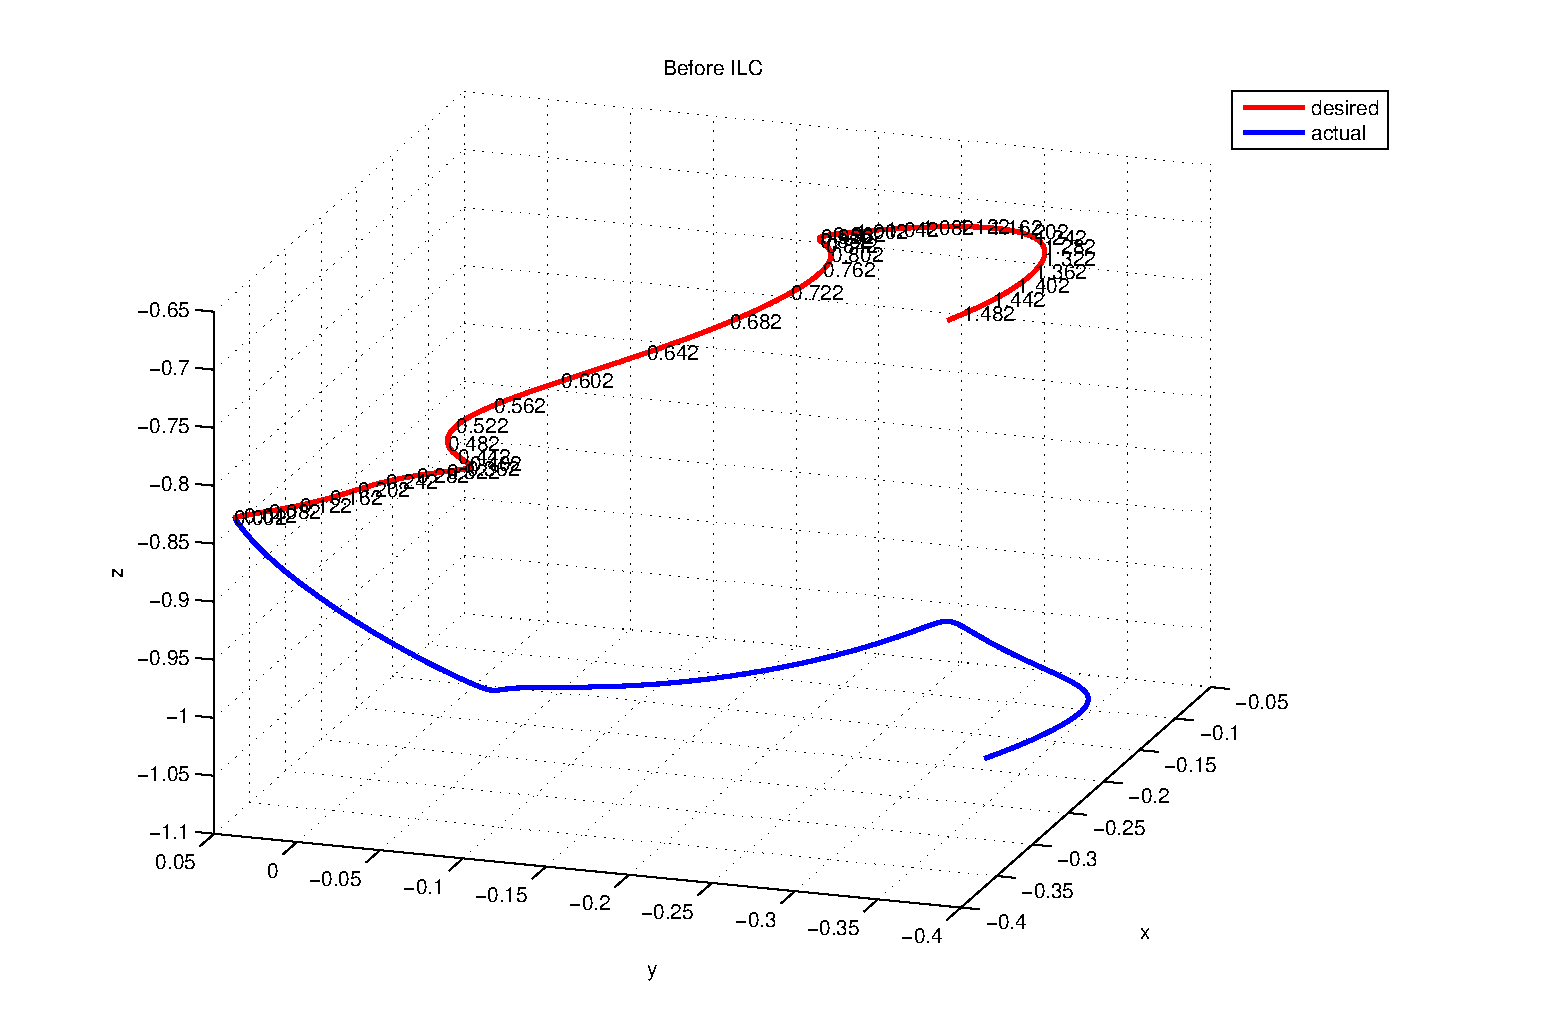
\includegraphics[width=\linewidth, height=0.15\textheight]{beforeILC.eps}
        \caption{(a)}
        \label{fig1}
    \end{minipage}%
    \begin{minipage}{.32\textwidth}
        \centering
        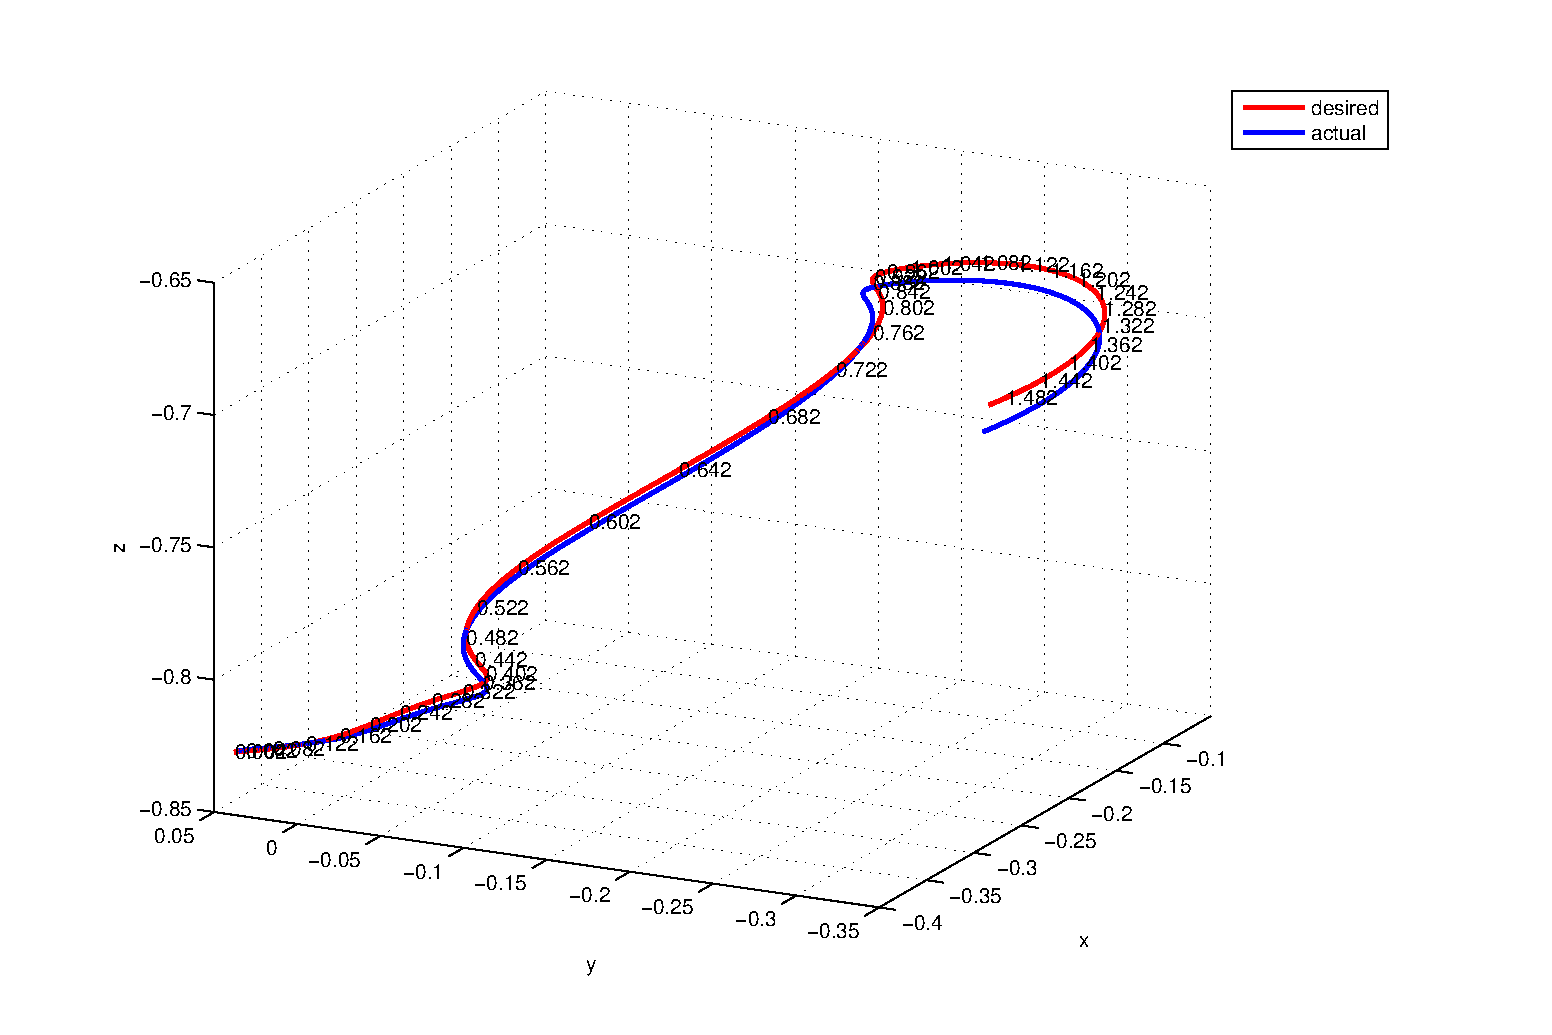
\includegraphics[width=\linewidth, height=0.15\textheight]{afterILCPseudoInv.eps}
        \caption{(b)}
        \label{fig2}
    \end{minipage}
    \begin{minipage}{.32\textwidth}
        \centering
        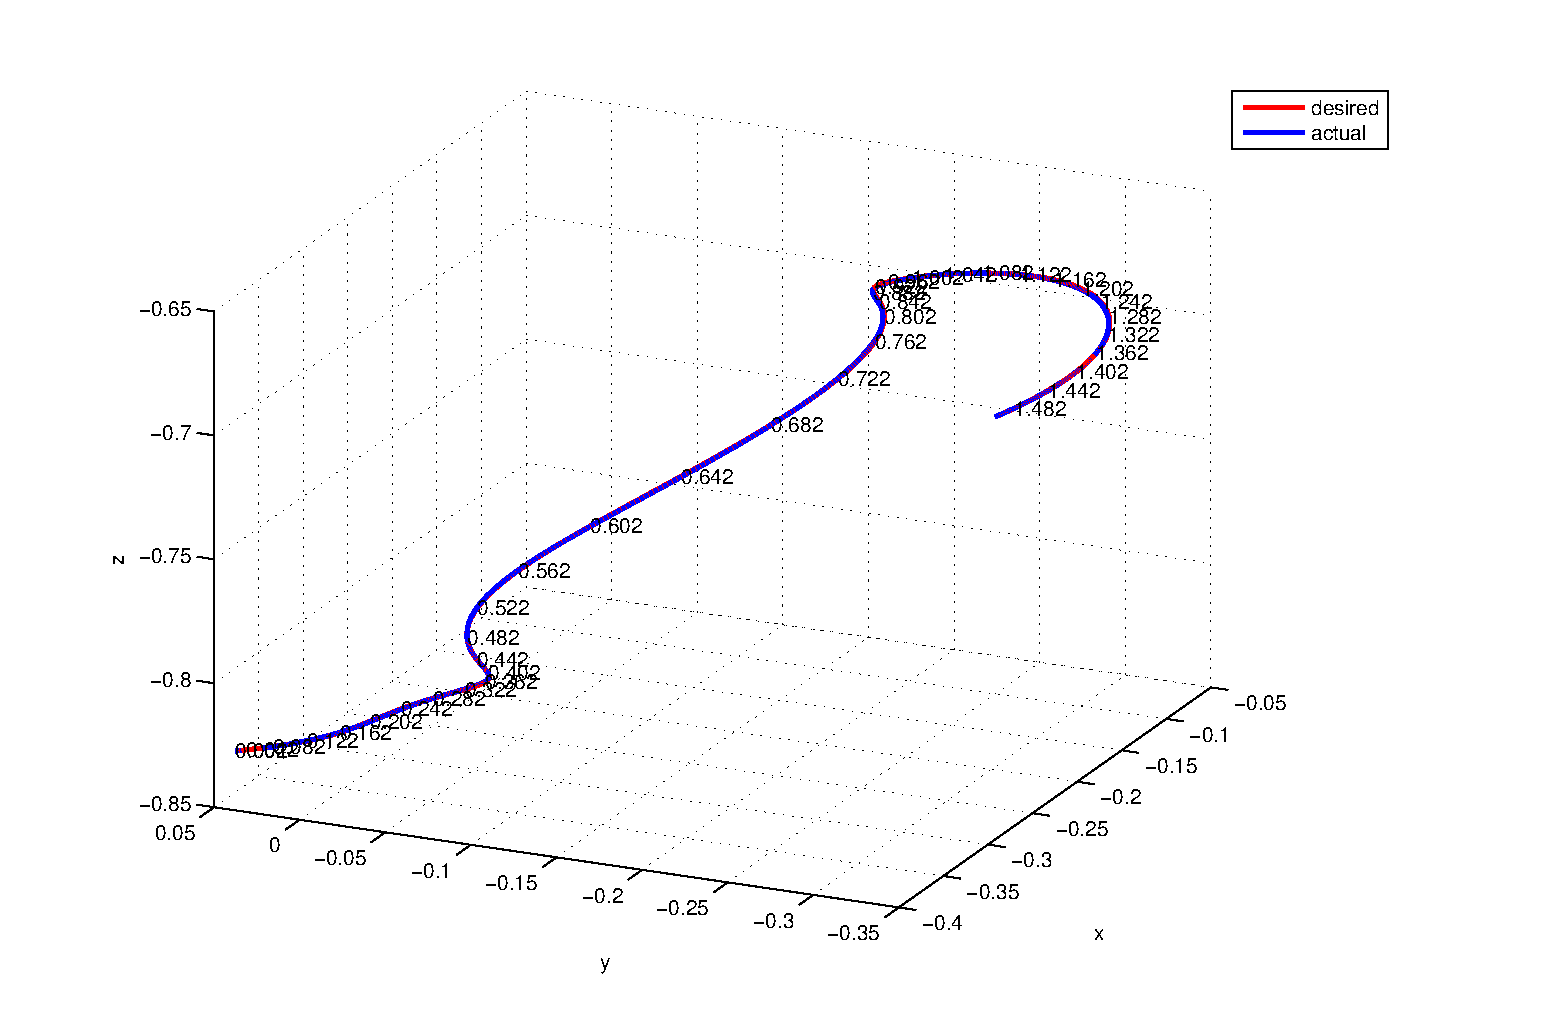
\includegraphics[width=\linewidth, height=0.15\textheight]{afterILCTLS.eps}
        \caption{(c)}
        \label{fig3}
    \end{minipage}
    \caption{Results showing the performance of trajectory tracking, before and after applying ILC (10 iterations). Reference trajectory is shown in red. Initially, in Figure~\ref{fig1}, tracking performance is poor. Final performances of pseudoinverse-based ILC and TLS-based ILC after learning are shown in Figures~\ref{fig2} and \ref{fig3} respectively. ILC with truncated pseudoinverse cannot approach the trajectory very well, and after 8 iterations starts to slowly diverge. ILC with truncated total least squares on the other hand approaches the trajectory very well, and shows excellent tracking performance that is also stable.}
\label{FigureILC}
\end{figure}

In the simulation results shown in Figure~\ref{FigureILC}, we consider a striking trajectory shown in red. Such ball-hitting trajectories in table tennis are generally composed of three parts: a preparatory phase, a hitting phase, and a relaxation phase. In the preparatory phase, the arm generally accelerates and picks up speed necessary to transfer the right momentum to the ball, intercepted in the hitting phase. The relaxation phase generally decelerates the arm and readies it for the next hitting task. 

ILC with pseudoinverse cannot approach trajectory very well, and after 8 iterations starts to slowly diverge. ILC with TLS on the other hand approaches the trajectory very well, and shows excellent tracking performance. For both methods, to be fair, we used the same truncation parameter, $\epsilon = 0.05$. This enables the pseudoinverse-based ILC to be more stable, i.e. without it ILC can show dangerous oscillations around some trajectories. However, even with truncation the pseudoinverse relies on the exactness of the model, whereas $\alg$ is inherently \emph{agnostic} to its accuracy. 

In practice we find that an additional adjustment in the form of \emph{current-iteration} ILC (\emph{CI-ILC}) 
%
\begin{equation}
\begin{aligned}
\sysInput_{k+1} &= \sysInput_k - \vec{K}_{LQR}\error_{k},\\
\end{aligned}
\label{fbILC}
\end{equation}
%
\noindent where we add the feedback from the previous iteration to the feedforward commands in the next iteration makes learning more robust. We add this current-iteration compensation to both methods in the results shown. 


\subsection{Applications in Robotic Table Tennis}

We performed the real robot experiments with a seven degree of freedom (DoF) torque-controlled custom made Barrett WAM arm capable of high speeds and accelerations.

\section{Conclusions and Future Work}\label{conclusions}

In this paper, we proposed a new ILC algorithm using total least squares (TLS), that is robust with respect to modeling uncertainties. Unlike most optimization and model-based approaches, our method is not overconfident. We proved that the proposed algorithm $\alg$ is agnostic to slight model mismatch, i.e. (monotonic) stability margins of ILC algorithms can be raised by using (truncated) TLS. Moreover we gave a Bayesian interpretation of our approach and built an adaptive Kalman-filter based routine that can adaptively identify the underlying latent matrix, and hence the dynamics model. Simulation and real robot results shown confirm the practical significance of our contributions. %incrementally or iteratively identify?

For future work, we would like to pursue the Bayesian interpretation of our algorithm further and in more detail. We believe that this way one can transcend the limitations of ILC and build a reinforcement learning (policy search) algorithm. By building locally and patching the underlying nonlinear dynamics model iteratively, the learning algorithm can learn between different trajectories. We plan to explore along this direction similarities to other model-based approaches and local regression techniques in the future.
% references needed : DDP and local regression.
% kernel and/or global TLS? 

\bibliographystyle{plain}
%\bibliographystyle{./IEEEtran}
%\bibliography{./IEEEabrv,./iros2015Ref}
\bibliography{./tempRef}

\end{document}
